\documentclass{article}
\title{Informe Técnico Proyecto Ciencia de Datos}
\author{Clàudia Hernández Bayés}
\date{July 2024}

\usepackage{geometry}
  \geometry{
  a4paper,
  total={170mm, 257mm},
  left=20mm,
  top=20mm,
    }
    
\usepackage{booktabs}

\usepackage{Sweave}
\begin{document}
\Sconcordance{concordance:Informetecnico.tex:Informetecnico.Rnw:1 15 1 1 0 12 1 1 11 %
19 0 1 2 3 1 1 21 1 2 3 1 1 46 28 0 1 2 3 1 1 24 13 0 1 3 1 1 1 18 1 2 %
5 1}


\maketitle
\tableofcontents


\section{Introducción}
El objetivo principal de este proyecto es analizar y comprender las tendencias, la prevalencia y los factores asociados con la discriminación en diversos contextos y grupos demográficos, con el fin de informar la formulación de políticas y estrategias que promuevan la igualdad y la inclusión social. A través del análisis de tendencias, buscamos identificar los patrones de discriminación en los últimos años y establecer una línea base que permita determinar el impacto de futuras intervenciones. Este enfoque nos permitirá detectar y responder a las tendencias emergentes de discriminación para prevenir la exclusión social.

Además, realizaremos un análisis demográfico para identificar y entender las áreas y los grupos demográficos donde la discriminación es más prevalente. Utilizando herramientas avanzadas de análisis de datos como R y Sweave, este estudio se propone elaborar un panorama detallado que refleje cómo varían los incidentes de discriminación según diferentes variables sociodemográficas. Este análisis profundo es crucial para el diseño de políticas efectivas que aborden las raíces y las manifestaciones de la discriminación en nuestra sociedad.


\section{Objetivo 1}
El objetivo primordial del proyecto es identificar y comprender las tendencias de discriminación a lo largo de los últimos años, utilizando un enfoque analítico detallado a través de gráficos de series temporales.

\subsection{Tabla Resumen}

% latex table generated in R 4.3.2 by xtable 1.8-4 package
% Wed Jul 24 14:46:12 2024
\begin{table}[ht]
\centering
\begin{tabular}{rr}
  \hline
essround & count \\ 
  \hline
2002 &  81 \\ 
  2004 &  71 \\ 
  2006 &  62 \\ 
  2008 &  89 \\ 
  2010 &  56 \\ 
  2012 &  65 \\ 
  2014 &  75 \\ 
  2016 & 119 \\ 
  2018 & 108 \\ 
  2020 & 286 \\ 
   \hline
\end{tabular}
\end{table}
En general, se observa una tendencia fluctuante en el número de casos de discriminación a lo largo de los años. A partir de 2014, hay un incremento significativo que alcanza su punto máximo en 2023 con 161 casos. Esto podría indicar un aumento en la concienciación y la denuncia de casos de discriminación, aunque también podría reflejar un incremento real en los incidentes de discriminación.En la siguiente gráfica podemos desglosar este recuento por tipo de discriminación. 

\subsection{Gráfico}
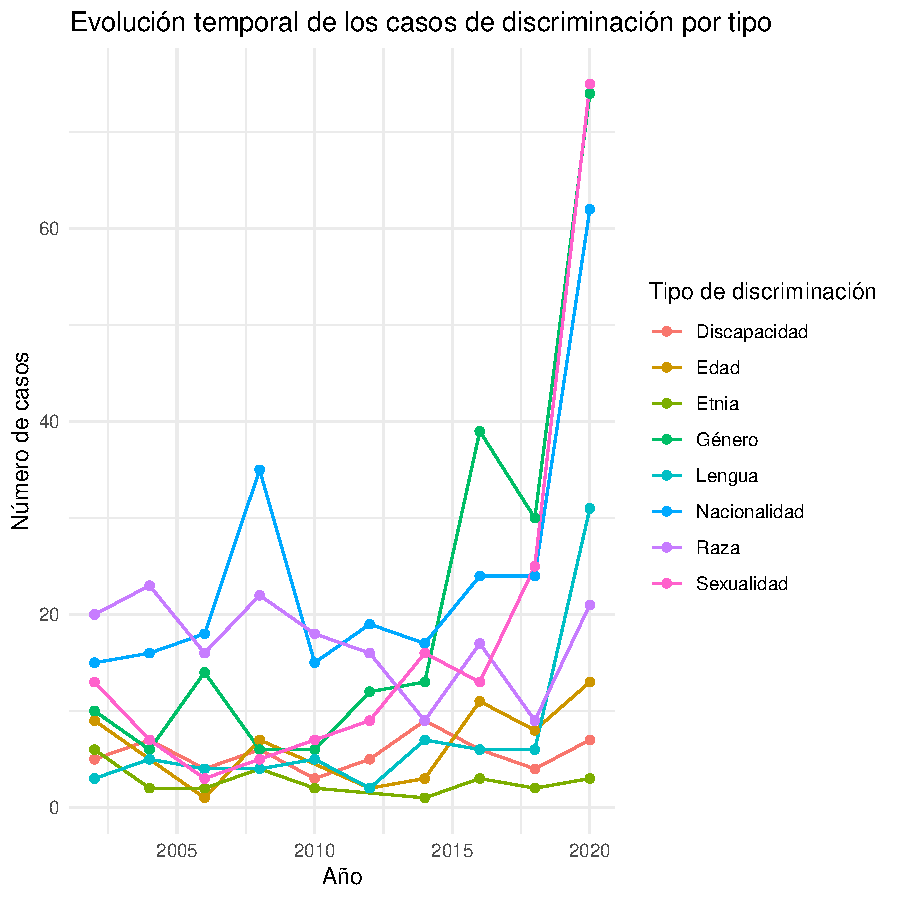
\includegraphics{Informetecnico-002}
Este tipo de gráfico es esencial para visualizar tendencias, detectar patrones y observar los efectos de eventos específicos en los datos. En este análisis, el eje X del gráfico representa el tiempo, dividido en períodos regulares que permiten una interpretación clara de la evolución temporal de la discriminación. El eje Y, por su parte, muestra la cantidad de casos reportados de discriminación, proporcionando una métrica directa del fenómeno.

Para una mayor comprensión de las dinámicas de la discriminación, el gráfico incorpora una codificación por colores que distingue entre diferentes tipos de discriminación, permitiendo comparaciones directas sobre cómo cada tipo varía en relación con los demás a lo largo del tiempo.

Generalmente, todos los tipos de discriminación aumentan entre 2002 y 2023, excepto por etnia. El crecimiento es exponencial en los casos de discriminación por sexualidad, nacionalidad y género, moderado por lengua y bajo por discriminación y edad. En concreto, la discriminación por sexualidad, nacionalidad y género supera el umbral de 60 casos en el año 2023, por lengua y raza se sitúan entre 20 y 40 y por edad, discapacidad y etnia se sitúan por debajo de los 20. 


\section{Objetivo 2}
El segundo objetivo de este proyecto es identificar las regiones de España donde la discriminación es más prevalente, medido como el número de casos de discriminación por cada 100,000 habitantes.

\subsection{Tabla Resumen}
% latex table generated in R 4.3.2 by xtable 1.8-4 package
% Wed Jul 24 14:46:12 2024
\begin{table}[ht]
\centering
\begin{tabular}{rrrr}
  \hline
region & casos & poblacion & tasa\_discriminacion \\ 
  \hline
Galicia &  47 & 2701743.00 & 1.74 \\ 
  Principado de Asturias &   9 & 1006193.00 & 0.89 \\ 
  Cantabria &  15 & 583904.00 & 2.57 \\ 
  País Vasco &  42 & 2188017.00 & 1.92 \\ 
  Comunidad Foral de Navarra &  11 & 661203.00 & 1.66 \\ 
  La Rioja &   7 & 319914.00 & 2.19 \\ 
  Aragón &  28 & 1320586.00 & 2.12 \\ 
  Comunidad de Madrid & 138 & 6714142.00 & 2.06 \\ 
  Castilla y León &  40 & 2394918.00 & 1.67 \\ 
  Castilla-La Mancha &  17 & 2046107.00 & 0.83 \\ 
  Extremadura &  11 & 1065424.00 & 1.03 \\ 
  Cataluña & 148 & 7739758.00 & 1.91 \\ 
  Comunitat Valenciana &  71 & 5057353.00 & 1.40 \\ 
  Illes Balears &  15 & 1172540.00 & 1.28 \\ 
  Andalucía &  81 & 8472403.00 & 0.96 \\ 
  Región de Murcia &  12 & 1511251.00 & 0.79 \\ 
  Ciudad de Ceuta &   1 & 84777.00 & 1.18 \\ 
  Ciudad de Melilla &   1 & 86384.00 & 1.16 \\ 
  Canarias &  15 & 2252465.00 & 0.67 \\ 
   \hline
\end{tabular}
\end{table}
La tabla proporciona una visión detallada de la distribución de casos de discriminación a lo largo de diversas regiones de España. Se destaca que Cantabria presenta la tasa de discriminación más alta con 2.57 casos por cada 100,000 habitantes, seguida por La Rioja con una tasa de 2.19, y Aragón con 2.12. En términos absolutos, Cataluña lidera con 148 casos reportados, seguida por la Comunidad de Madrid con 138 casos, y Andalucía con 81. Estos números indican que, aunque algunas regiones tienen grandes poblaciones y, por ende, más casos en total, las tasas de discriminación pueden variar significativamente, sugiriendo que la incidencia de la discriminación no es homogénea en todo el país.

Por otro lado, algunas regiones presentan tasas de discriminación considerablemente bajas. Canarias muestra la tasa más baja con 0.67 casos por cada 100,000 habitantes, seguida de Castilla-La Mancha con 0.83, y la Región de Murcia con 0.79. Es notable que ciudades con pequeñas poblaciones, como Ceuta y Melilla, aunque reportan solo un caso cada una, tienen tasas relativamente altas debido a sus pequeñas poblaciones (1.18 y 1.16, respectivamente). En general, la variación entre las tasas y los números absolutos de casos sugiere diferencias regionales significativas en la prevalencia de la discriminación, la disposición a reportar incidentes, o ambos factores.


\section{Objetivo 3}
El tercer objetivo de nuestro proyecto se centra en explorar la relación entre ciertas variables demográficas y la incidencia de casos de discriminación. En particular, hemos seleccionado la variable que indica si los participantes han tenido o no un trabajo pagado a lo largo de su vida. Esta variable es significativa porque el empleo es a menudo un área donde las desigualdades y la discriminación pueden ser más evidentes y tener impactos más profundos en la vida de las personas.


\subsection{Tabla Resumen}
% latex table generated in R 4.3.2 by xtable 1.8-4 package
% Wed Jul 24 14:46:12 2024
\begin{table}[ht]
\centering
\begin{tabular}{ccrr}
  \hline
pdjobev & discriminado & count & percentage \\ 
  \hline
Sí & No & 6050 & 95.61 \\ 
  Sí & Sí & 278 & 4.39 \\ 
  No & No & 2738 & 94.87 \\ 
  No & Sí & 148 & 5.13 \\ 
   \hline
\end{tabular}
\end{table}La tabla presentada proporciona una visión clara sobre la relación entre haber tenido un trabajo pagado (pdjobev) y haber experimentado discriminación (discriminado). Los resultados se dividen en cuatro categorías que combinan ambas variables, mostrando tanto el número de casos (count) como el porcentaje correspondiente (percentage).

Entre los participantes que han tenido algún trabajo pagado (Sí), un 95.61 por ciento (6050 casos) no ha experimentado discriminación, mientras que el 4.39 por ciento (278 casos) sí ha sido discriminado. Esto indica que la gran mayoría de las personas con experiencia laboral remunerada no ha enfrentado discriminación, aunque existe una minoría significativa que sí la ha sufrido.

Por otro lado, entre aquellos que nunca han tenido un trabajo pagado (No), un 94.87 porciento (2738 casos) no ha sido discriminado, y un 5.13 por ciento (148 casos) sí ha experimentado discriminación. Aunque la proporción de discriminación es ligeramente mayor en este grupo en comparación con los que han tenido un trabajo pagado, la mayoría sigue sin haber enfrentado discriminación. En general, estos datos sugieren que, si bien haber tenido un trabajo pagado no parece estar fuertemente asociado con la experiencia de discriminación, hay una ligera variación en las tasas de discriminación entre los dos grupos.



\subsection{Gráfico}
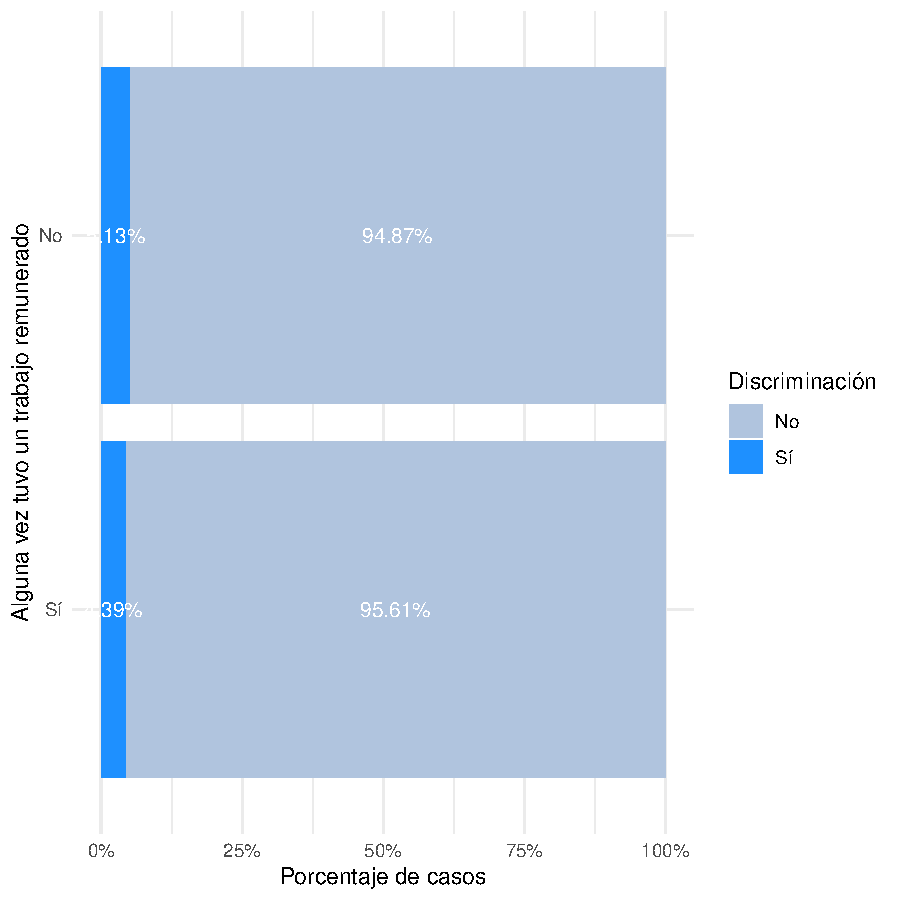
\includegraphics{Informetecnico-005}


\section{Conclusiones}
Las conclusiones derivadas de este análisis profundo sobre las tendencias y prevalencia de la discriminación en diferentes contextos y grupos demográficos, utilizando herramientas avanzadas como R y Sweave, proporcionan insights valiosos para el diseño de políticas y estrategias efectivas que promuevan la igualdad y la inclusión social. A continuación, se resumen los hallazgos más significativos:

\begin{enumerate}
\item Entre 2002 y 2023, se observa un aumento general en todos los tipos de discriminación, excepto por etnia. La discriminación por sexualidad, nacionalidad y género ha crecido exponencialmente, superando los 60 casos en 2023.
\item La discriminación varía significativamente entre regiones, con Cantabria, La Rioja y Aragón presentando las tasas más altas. Cataluña y Madrid tienen los números absolutos de casos más altos.
\item La mayoría de las personas con trabajo pagado no ha enfrentado discriminación (95.61 por ciento), mientras que aquellos sin experiencia laboral tienen una ligera mayor incidencia (5.13 por ciento).
\end{enumerate}

\end{document}
